%!TEX root = ../Thesis.tex
\section{Electrocardiogram (ECG)}
Electrocardiography is a non-invasive method of recording the electrical activity of the heart. This is achieved by positioning leads/ electrodes on the body in standardized location. The tiny electrical changes during a heartbeat creates an electrophysiologic pattern of depolarizing and repolarizing.
The graph of voltage of electrical signal created during the heartbeat versus time is called Electrocardiogram (ECG). Each cardiac cycle is represented by a sinus rhythm. The word ‘rhythm’ is used to refer to the part of the heart which is controlling the activation sequence. The normal heart rhythm, with electrical activation beginning in the Sinoatrial node, is called ‘sinus rhythm’.\cite{hampton_ecg_2013}

\begin{figure}
	\centering
	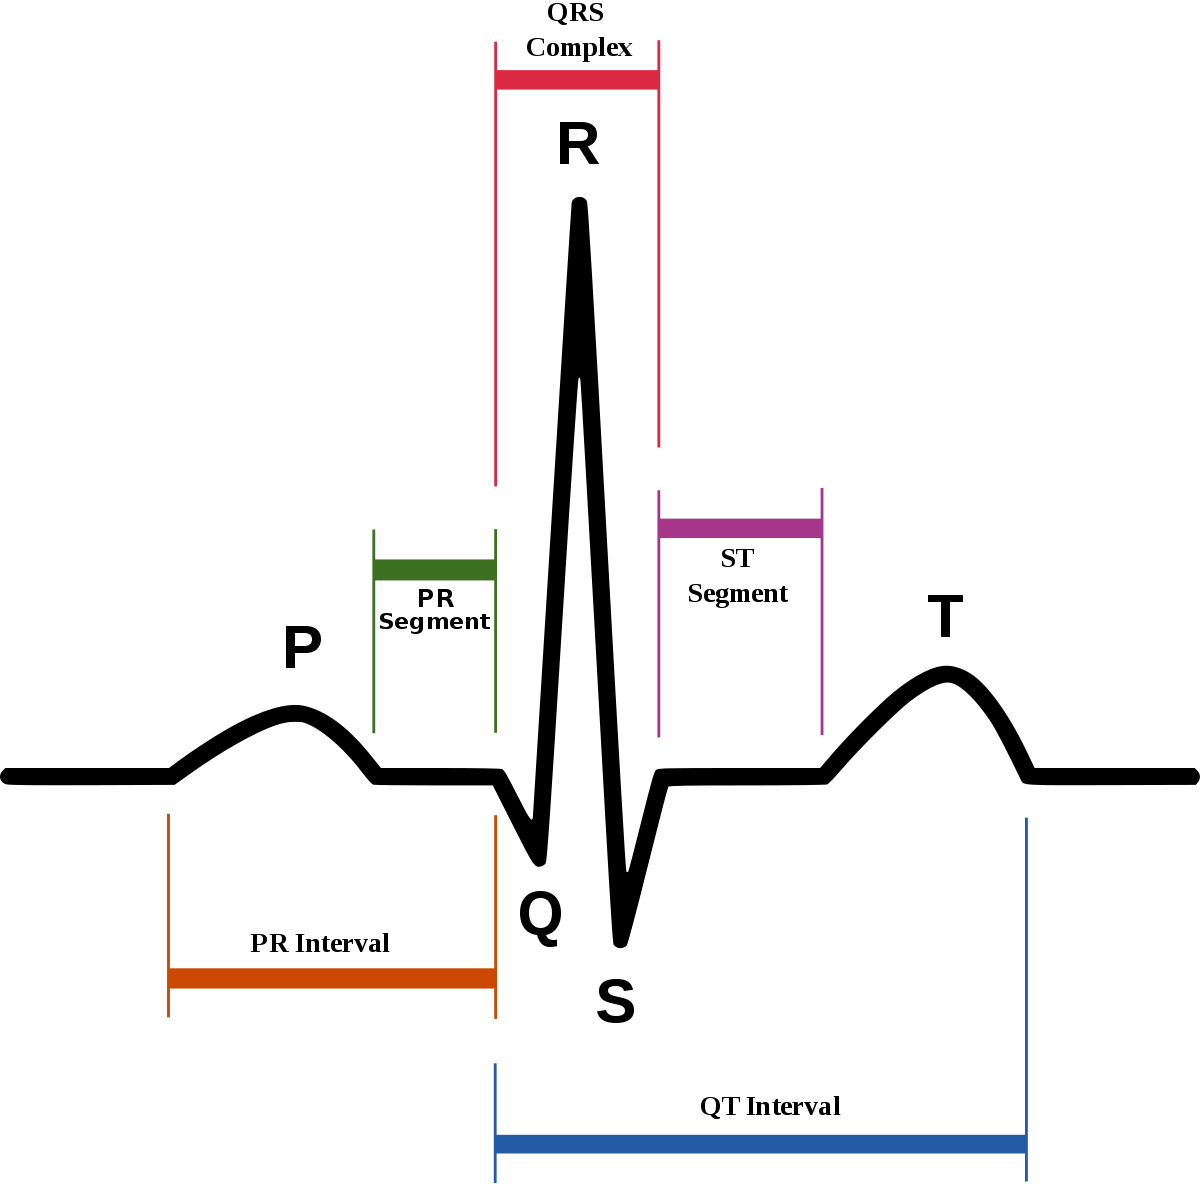
\includegraphics[width=100mm]{SinusRhythmLabels.png}
	\caption{Sinus Rhythm Labels}
	\label{fig:sinus_rhythm_labels}
\end{figure}

\subsection{Normal Sinus Rhythm (NSR)}
A Normal Sinus Rhythm is used to denote a Sinus Rhythm of a healthy functioning heart. The Normal Sinus Rhythm (NSR) can be schematically represented in standard wave form as showing in fig. Different points on the wave are represented by a letter. The letters P, Q, R, S and T were selected in the early days of ECG history and were chosen arbitrarily. [ref book] The segment between three of graphical deflections - Q, R and S points in the waveform forms a QRS Complex.

\subsection{QRS Complex}
QRS Complex has a lot of clinical significance. QRS complex are useful in diagnosing cardiac arrhythmias, conduction abnormalities, ventricular hypertrophy, myocardial infarction, electrolyte derangements, and other disease states.\cite{noauthor_qrs_2018}
\paragraph{}
QRS Complex has also been utilized by several researchers to extract features to detect emotions. For example, J Kim et al. were able to extract features in time and frequency domain to recognize emotions in music listening.\cite{kim_emotion_2004}

\subsection{R-R Interval}
R-R interval is distance between peaks of two consecutive sinus rhythm. This distance between two R-peaks is used to determine the Heart Rate Variability (HRV).

\todo{Add a more descriptive description of R-R Interval}

\section{Electrodermal Activity}
Electrodermal Activity (EDA) is defined as autonomic change in the skin conductance which is quantified by applying an electrical potential between two points of contact and measuring the resulting current flow between them. Electrodermal Activity (EDA) is measured by placing two leads/electrodes in standardized position of the body and then measuring the resistance.
\paragraph{}
Sweat gland secretion is a process which helps regulate temperature in body. Whenever, aroused or relaxed this state is reflected upon the sweat inhibition at glands on palms or feet, changing the resistance of the skin. Thus, Electrodermal Activity (EDA) has been widely utilized for determining arousal and emotion processing.

\begin{figure}
	\centering
	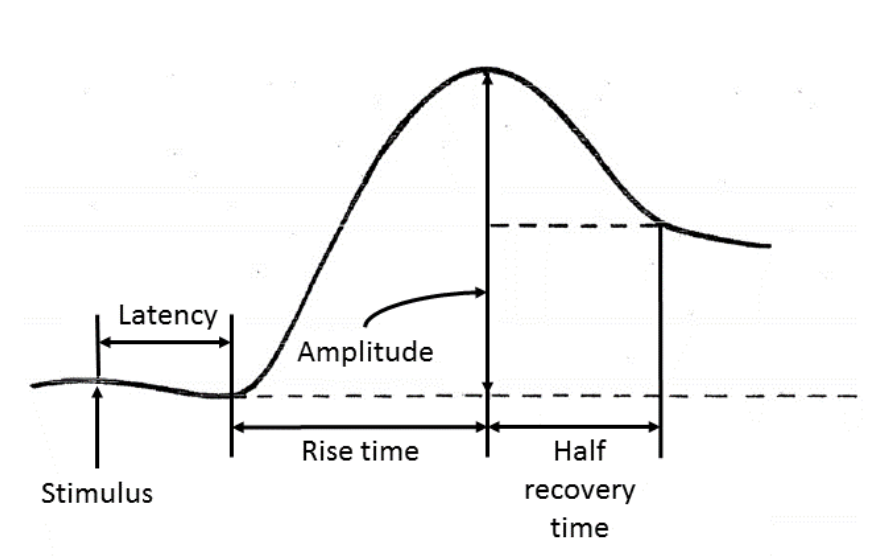
\includegraphics[width=100mm]{eda_graph.png}
	\caption{Time-domain measures of EDA based on the specific SCR caused by an instantaneous stimulus}
	\label{fig:eda_graph}
\end{figure}

Figure \ref{fig:eda_graph} shows a time-domain typical time-domain measure of EDA due to Skin Conductance Response (SCR), because of instantaneous stimuli. The SCR’s stimulus-onset latency, amplitude and rise time are used to assess the level of stress induced by stimuli. 






